\chapter{数据集}\label{dataset}
CLEVR作为空间推理领域的重要数据集,极大地推动了视觉问答的发展,
对人工智能的研究、教学等方面的发展具有重要影响。
尽管如此,CLEVR主要关注完全可见的场景,不能反映部分可见场景在现实世界中广泛存在的情况。
因此,本章将基于CLEVR数据集,并参考Liang\cite{liang2022visualabductivereasoning}等人的研究,
引入部分可见场景、遮挡机制与复杂空间关系,以全面考察模型在部分可见场景中回答空间推理问题的能力。

\section{设计目标}
本章旨在构建一个积木世界部分可见场景空间推理数据集(Partial Observation VQA Data\-set, POVQAD)
,以有效评估本文后续提出的面向空间推理的神经符号VQA框架的性能。
现有的一些空间推理数据集(例如经典反映积木世界的CLEVR数据集)通常假设场景完全可见,这与现实世界的环境存在显著差异。
在真实物理环境中,智能体往往只能通过有限的传感器(如摄像头、激光雷达)获取关于环境的部分信息,面临着遮挡、视野限制等挑战。
部分可见性是智能体执行导航、抓取和交互任务时必须处理的核心问题之一。因此,构建一个包含部分可见场景的空间推理数据集,
对于评估和提升智能体在部分可见场景中的空间推理能力至关重要,也是人工智能的研究、教学等方面进一步发展的先决条件。

为了弥补现有数据集与实际应用场景之间的差距,并提升模型在部分可见场景下的空间推理能力,本数据集引入部分可见性,
借鉴Liang\cite{liang2022visualabductivereasoning}的研究,在数据集中引入部分可见的场景,
模拟现实中因遮挡、视角受限等引起的信息缺失。
在实现层面上,可通过程序化生成包含不同程度遮挡或信息缺失的三维场景及其对应的多种视角图像或状态描述。
最终,使数据集能够评估模型在信息不完整条件下进行空间推理的能力,例如推断被遮挡物体的位置、属性或存在性。

\section{物体属性}
POVQAD 数据集中每个图像中的物体均具有形状、尺寸、材质和颜色四种属性。每种属性的可能取值如下:
\begin{enumerate}[label=(\arabic*),itemsep=0pt,parsep=0pt]
    \item 形状:圆锥体、球体、圆柱体和立方体。
    \item 尺寸:小、中、大。
    \item 材质:橡胶、金属。
    \item 颜色:红色、蓝色、绿色、黄色、灰色、棕色、紫色、青色。
\end{enumerate}

选择颜色、形状、材质和大小这四个基本视觉属性,是因为它们是物体最直观且容易区分的特征,并且与原始CLEVR数据集保持一致,便于进行比较研究。
对每个属性的可能取值进行了限制(例如,八种颜色,四种形状,两种材质,三种尺寸),这样做的目的是为了简化推理过程并控制答案的搜索空间 。

除上述四种基本属性之外,图像中的物体也具有“区域”这一属性,其取值为 0、1、2、3。由于所有图像都被划分成
4个区域,故图像中物体也会处在某一个区域之中。为了研究问题方便,本文规定每个物体只能在图像的一个区域中,不能
同时跨多个区域。物体包含这一属性能够为指定约束提供便利。在本数据集中,约束是一组规则的集合,对场景生成
与推理而言密不可分,其主要作用包括:(1)限制物体的属性组合,如对颜色、形状等进行限制;
(2)定义物体之间的关联关系;(3)支持对遮挡物体的推理,当物体被遮挡时,通过约束可以缩小潜在答案的范围。

基于对物体的应用范围,约束可以划分为以下三类:
\begin{enumerate}[itemsep=0pt,parsep=0pt]
    \item 区域约束:仅作用于特定区域的局部规则。例如,“区域1中所有物体形状必须为立方体”。
    \item 跨区域约束:涉及多个区域的全局规则。例如,“区域1和区域2中同颜色物体的总数不超过2个”。
    \item 全局约束:适用于整个场景的通用规则。例如,“所有物体必须属于至少一个区域”或“不允许存在完全相同的两个物体属性组合”。
\end{enumerate}

约束通过使用ASP来进行表示。例如:
\begin{lstlisting}
    :- obj(X), at(X, 0), not has_property(X, shape, cube), not has_property(X, shape, cylinder).
\end{lstlisting}
表示如果X在区域0,那么它的形状必须是立方体或圆柱体。

将区域属性引入到物体上,使得可以在不同层面上定义约束。这就要求模型在进行推理时,需要考虑物体之间的空间关系以及约束在不同区域的应用,增加了推理任务的复杂性。
\section{构建过程}
\subsection{环境生成}
环境生成是构建POVQAD数据集的第一步,其目的是定义一个具有领域特定约束的“环境”,为场景中物体的属性和空间分布提供先验限制。
POVQAD中的环境是由一组约束来定义的。本文选择使用ASP对约束进行表示。
ASP是一种声明式逻辑编程范式,非常适合表示知识和进行推理。数据集中使用了11种不同的约束模板,
每个环境通过实例化最多15个模板来完成创建,并且保证每个场景区域至少有两个约束。
部分约束模板的ASP编码表示以及对应表示含义见表\ref{tab:asp_templates}。最终,一共生成了30个
环境,数据集中的所有场景均匀分布在这些不同的环境之中。环境的具体示例见附录\ref{appendix:environment}。

使用ASP来定义环境和约束,为场景的生成和推理评估提供了一个正式且逻辑严谨的框架。
通过改变约束的数量和类型,数据集可覆盖多种场景规,从而增加了数据集的多样性和复杂性,避免模型仅仅学习到特定环境下的模式而缺乏泛化能力。
\begin{table}[h]
    \centering
    \renewcommand{\arraystretch}{1.0}
    \begin{tabular}{|p{3cm}|p{12cm}|}
        \hline
        \textbf{模板} & \textbf{描述} \\
        \hline
        \textbf{模板1(取值约束)} & 
        \texttt{:- obj(X), at(X, R), not has\_property(X, P1, V1).} \\ 
        & 解释: 对区域R中的所有物体,它们P1属性的取值均为V1。 \\ 
        & 具体实现: :- obj(X), at(X, 0), not has\_property(X, color, red). \\
        \hline
        
        \textbf{模板2(否定约束)} & 
        \texttt{:- obj(X), at(X, R), has\_property(X, P1, V1).} \\ 
        & 解释:对区域R中的所有物体,它们的P1属性的取值,均不能为V1。 \\ 
        & 具体实现::- obj(X), at(X, 0), has\_property(X, material, metal). \\
        \hline
        
        \textbf{模板3(恰有N个约束)} & 
        \texttt{:- \#count\{X: has\_property(X, P1, V1), obj(X), at(X, R)\} != N.} \\ 
        & \textbf{解释}:在区域R中,恰好有N个物体的P1属性的取值为V1。 \\ 
        & 具体实现::- \#count\{X: has\_property(X, size, small), obj(X), at(X, R')\} != 2. \\
        \hline
        
        \textbf{模板4(至少有N个约束)} & 
        \texttt{:- \#count\{X1, X2: sameProperty(X1, X2, P1), obj(X1), obj(X2), at(X1, R1), at(X2, R2)\} < N.} \\ 
        & 解释:在区域R1和区域R2中,至少有N对物体,它们的P1属性的取值都是V1。 \\ 
        & 具体实现::- \#count\{X1, X2: sameProperty(X1, X2, shape), obj(X1), obj(X2), at(X1, 1), at(X2, 2)\} < 1. \\
        \hline
        
        \textbf{模板5(或约束)} & 
        \texttt{:- obj(X), at(X, R), not has\_property(X, P1, V1), not has\_property(X, P1, V2).} \\ 
        & 解释:区域 R中的所有对象都具有属性 P1 的 V1 值或属性 P2 的 V2 值。 \\ 
        & 具体实现::- obj(X), at(X, 1), not has\_property(X, color, yellow), not has\_property(X, color, blue). \\
        \hline
    \end{tabular}
    \caption{部分约束模板示例}
    \label{tab:asp_templates}
\end{table}
\subsection{完整场景图生成}
完整场景图生成是POVQAD数据集构建的第二步,其目的是在给定的环境约束下生成完整的场景图,确保所有物体的属性(颜色、形状、尺寸和材质)以及空间关系均满足预定义约束。
成功定义一个环境的约束之后,下一个步骤是生成一个符合这些约束的完整场景图$Complete_i$。
这个场景图描述了场景中所有物体的属性,包括颜色、大小、形状和材质,以及它们在四个预定义区域中的位置。
生成过程的关键在于确保场景图中的每一个物体及其属性的赋值都与当前环境的所有约束相一致。
为了达到以上目的,本文在此处使用ASP来进行生成,以环境的约束和期望生成的物体数量作为ASP求解器的输入,通过求解器来找到所有可能的有效物体配置。
每一个满足所有约束的物体配置都被视为一个有效的场景图。
为了后续的图像生成,研究人员随机抽样了数百万个这样的完整场景图。
通过这种方式生成的完整场景图保证了场景内部逻辑上的一致性,
为后续引入部分可观察性以及生成问题奠定了坚实的基础。随机抽样大量的有效场景图也有助于增加数据集的规模和多样性。   

以下\ref{asp:scene}为对场景使用ASP进行表示的示例。
\begin{lstlisting}[label=asp:scene]
%场景中的物体
obj(0). obj(1). obj(2). obj(3).

%物体的属性
at(0, 2).
has_property(0, color, green).
has_property(0, size, large).
has_property(0, material, rubber).
has_property(0, shape, cylinder).
....

%物体间的空间关系
front(1, 0). right(1, 0). ...
\end{lstlisting}

其中涉及到的谓词的功能如下:谓词\texttt{obj}用于定义不同的物体(所有物体的名称用0,1等数字来表示)。
谓词\texttt{has\_property(obj, Attribute, Value)}用于将对象的名为Attribute的属性的值设置为Value。
对象之间的空间关系用谓词\texttt{left}、\texttt{right}、\texttt{front}、\texttt{behind}来表示,例如
\texttt{left(A, B)}表示B位于A的左侧。

最后,在图\ref{pipeline_for_generating_environment}直观展示了从环境约束到该环境中场景图构建的过程。
\begin{figure}
    \centering
    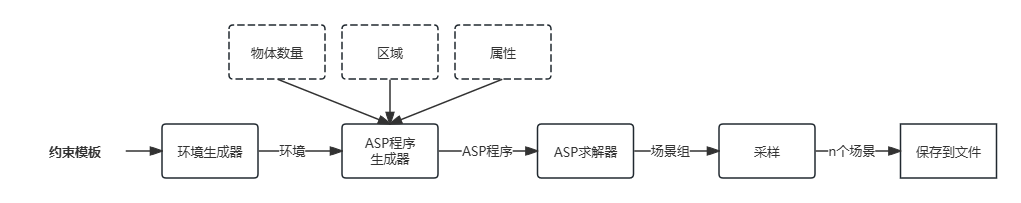
\includegraphics[width=\textwidth]{pipeline_for_generating_environment.png}
    \caption{生成环境以及该环境中的完整场景的流水线}
    \label{pipeline_for_generating_environment}
\end{figure}
\subsection{部分场景图生成}
部分场景图生成是POVQAD数据集构建的第三步,其目的是从完整场景图中故意移除目标物体,构建信息缺失的场景实例,以模拟部分可见场景。
为了引入部分可观察性,本文从每个完整的场景图$Complete_i$中随机移除一个物体$Obj_i$,从而创建了一个部分场景图$Partial_i$。
这个被移除的物体将成为后续问题关注的“隐藏”对象 。
这种通过移除单个物体来创建部分场景的方法不仅相对简单,而且有效地模拟了现实世界中物体被遮挡或不可见的情况。
剩余的可见物体以及环境的约束将成为推断隐藏物体属性的关键信息来源。这种设计选择使得推理任务更加明确和集中。
\subsection{问题与答案生成}
问题与答案生成是POVQAD数据集构建的第四步,其目的是围绕被隐藏的物体构建自然语言问题,并生成与之对应的符号表示,供推理模块使用。
POVQAD数据集中的视觉问题$Q_i$专门针对部分场景中被移除的隐藏对象。这些问题旨在查询该隐藏对象的四个属性之一:颜色、尺寸、形状或材质 。
为了生成这些问题,本文借鉴了原始CLEVR数据集中的问题模板,但进行了修改,使其仅包含属性查询模板,并排除了是非题和计数题。
一种供参考的示例模板如\ref{asp:question-template}中所示,
其中<Z2>、<C2>、<M2> 表示待查询对象的已知属性(例如尺寸、颜色、材质),由随机策略从完整场景图中选取;
<R> 为空间关系(如left、right、front、behind),其取值既满足随机性,又依赖于完整场景中物体间的真实空间分布;
<Z>、<C>、<M>、<S> 则代表参考对象的属性,通过对完整场景图中与查询对象具有特定空间关系的候选对象进行筛选而确定。
这种模板化设计不仅使自然语言问题的结构化描述成为可能,而且便于后续转换为ASP的形式化表示,从而实现问题求解的自动化。

\begin{lstlisting}[label=asp:question-template]
What shape is the < Z2 > (size) < C2 > (color) < M2 > (material) [that is] 
< R > (relation) the < Z > (size) < C > (color) < M > (material) < S > (shape) ?
\end{lstlisting}

问题的生成过程基于完整的场景图,并且被查询的属性是经过精心选择的,以保证不同问题类型之间的平衡。
具体步骤包括:
\begin{enumerate}[itemsep=0pt,parsep=0pt]
\item 场景图构建与部分场景生成。利用完整场景图构建方法,将真实场景中的物体、属性以及空间关系进行抽象建模;
从完整场景中随机移除一个物体,以构造部分场景图,此移除的对象即为“查询对象”,其缺失的属性将作为问题求解目标。
\item 已知属性的随机选取。对于查询对象,模板中的已知属性(例如<Z2>、<C2>、<M2>)由随机采样策略确定,
确保不同问题之间在属性分布上具有较好的随机性和代表性;同时,选取的属性应满足数据集整体的“问题类型平衡”要求,避免某一属性出现频率过高或过低。
\item 空间关系的确定。对于模板中表示空间关系的部分(<R>),取值虽然随机,但参考对象的选择依赖于完整场景图中的物体空间布局。
具体而言,从与查询对象存在 <R> 关系的物体中进行候选对象的筛选,从而确保问题中提及的空间关系具有实际语义意义。
\end{enumerate}

在问题生成过程中,一个重要的设计原则是,生成的问题必须满足解的数量$S$大于等于1且小于被查询属性的所有可能值的总数$|A|$ 。
例如,如果查询的是大小属性(共有三个可能值:大、中、小),那么问题的答案可以是{大,中},{大,小},{小,中},{大},{中}或{小},
而不能是包含所有三个值的集合。如果一个问题的所有可能值都是潜在答案,那么这个提问就被认为是无效的。
这种设计确保了模型需要通过推理来排除不一致的选项,而不是简单地猜测所有可能的属性值。

为了使问题具有可操作性和求解性,所有生成的问题均转化为ASP形式。转换过程中包括以下步骤:
\begin{enumerate}
\item 规则构建。将自然语言问题中的各项约束(属性约束、空间关系约束、对象排他性约束等)以ASP规则的形式表达;
\item 约束整合。同时将部分场景图与环境约束作为求解器的输入,确保问题求解过程在完整逻辑下进行;
\end{enumerate}

POVQAD数据集中问题的答案是通过Clingo求解器生成的 。
对于每一个问题,Clingo求解器会接收三个关键输入:以ASP形式表示的问题、以ASP形式表示的不完整场景以及定义当前环境的约束规则(也以ASP形式表示) 。
例如,问题“与中等大小的红色物体的材质相同的,另一个圆柱体的颜色是什么?” 
可以被表示为如下的ASP查询:
\begin{lstlisting}
query(Q) :- has_property(X, color, Q),
has_property(X, shape, cylinder),

has_property(Y, size, medium),
has_property(Y, color, red),
same_material(Y, X),
X != Y.
\end{lstlisting}
不完整的场景则会列出所有可见物体的属性(颜色、形状、材质、大小)以及它们所在的区域和彼此之间的空间关系(例如,在…前面,在…右边) 。
环境约束则定义了场景中物体属性和关系必须遵循的逻辑规则 。
ASP求解器利用这些输入进行逻辑推理,找出所有与给定的约束和部分场景信息相一致的、关于隐藏物体被查询属性的可能取值 。
这个过程通常涉及到排除法,即通过已知的知识排除掉不符合条件的可能性。最终,ASP求解器的输出是一个包含所有合理答案的集合。
由于问题是关于隐藏对象的,因此答案通常不是唯一的,而是一组可能的属性值。
例如,对于一个关于红色橡胶球的问题,ASP求解器可能得出答案为{小,中},这意味着根据当前的场景和约束,该隐藏物体的大小可能是小或者中 。
\subsection{图像生成与表示转换}
图像生成与转换是POVQAD数据集构建的最后一步,其目的是将生成的场景图转换为视觉图像,为视觉问答任务提供图像输入。
POVQAD数据集中的图像是从已知符合环境约束的场景图生成的。本文使用Blender这款3D建模和渲染软件来渲染场景图。
Blender3 是一款高效且功能丰富的三维渲染软件,它能够基于场景图的结构信息生成逼真的图像。
渲染过程包括以下几个关键步骤:(1)场景搭建,根据场景图中各物体的位置信息及属性参数,在 Blender3 中自动搭建三维场景;
(2)光照与材质设置,对各物体的材质、光照、纹理等进行设置,确保渲染出的图像在视觉上具有真实感;(3)
图像生成,利用 Blender3 的渲染引擎,将搭建好的场景生成最终图像。
然后,通过移除完整场景图中的一个物体,即可得到部分场景图,并基于这个部分场景图生成最终在数据集中呈现的图像。
这种图像生成方式保证了视觉输入与场景的底层逻辑表示之间存在直接的对应关系。

为了更全面地评估模型的性能,POVQAD数据集中的问题不仅包含自然语言形式,还提供了对应的ASP表示 。
这种双重表示使得模型既需要理解自然语言问题,又能够利用逻辑推理来找到答案。
ASP 问题表示、不完整的场景描述以及环境约束共同作为输入交由 ASP 求解器处理,从而确定问题答案。
\subsection{小结}
图\ref{pipeline_for_generating_partial}展示了构建POVQAD数据集的全过程。
该流程通过随机采样,使生成的问题在属性组合和空间关系上呈现多样性;通过对解集规模的判定机制,
有效过滤掉普遍适用或无区分意义的问题,确保每个问题都能够准确反映场景中物体属性的关系;
使用模板化设计和ASP表示为后续数据集扩充与新问题类型的加入提供了灵活性和统一标准。
\begin{figure}[h]
    \centering
    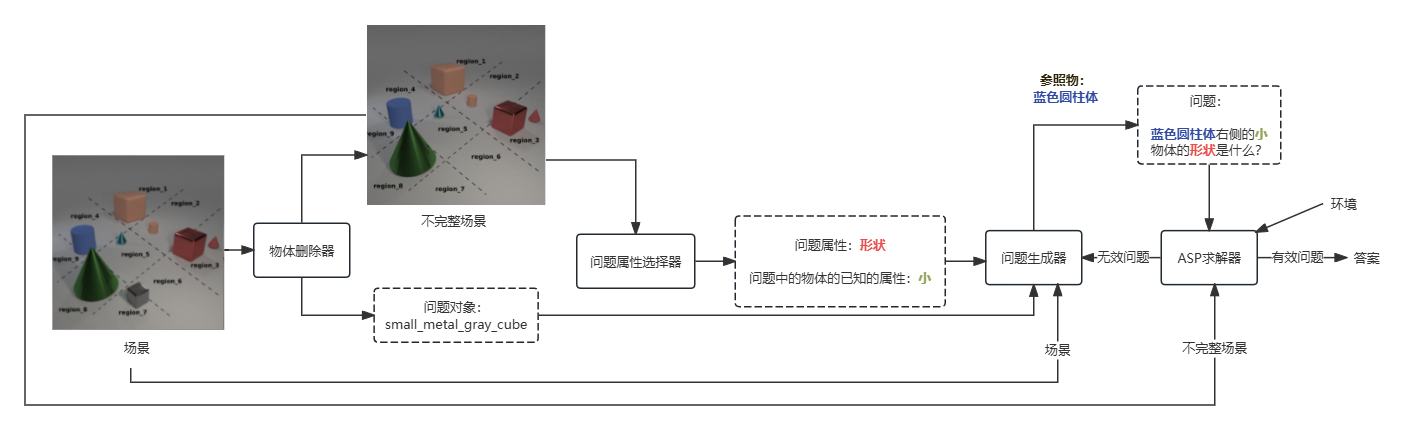
\includegraphics[width=\textwidth]{pipeline_for_generating_partial.png}
    \caption{生成部分场景和问题,并进行标记的流程}
    \label{pipeline_for_generating_partial}
\end{figure}
\section{数据集统计}
图\ref{fig:template_statistics}展示了问题模板分布及查询属性数量在 5 至 9 之间的统计结果。
本数据集是基于CLEVR数据集进行生成的,在问题模板方面,采用了CLEVR数据集中的六种问题模板。此外,也展示
了特定类型的问题在不同场景物体数量下的分布情况。
\begin{figure}[h]
    \centering
    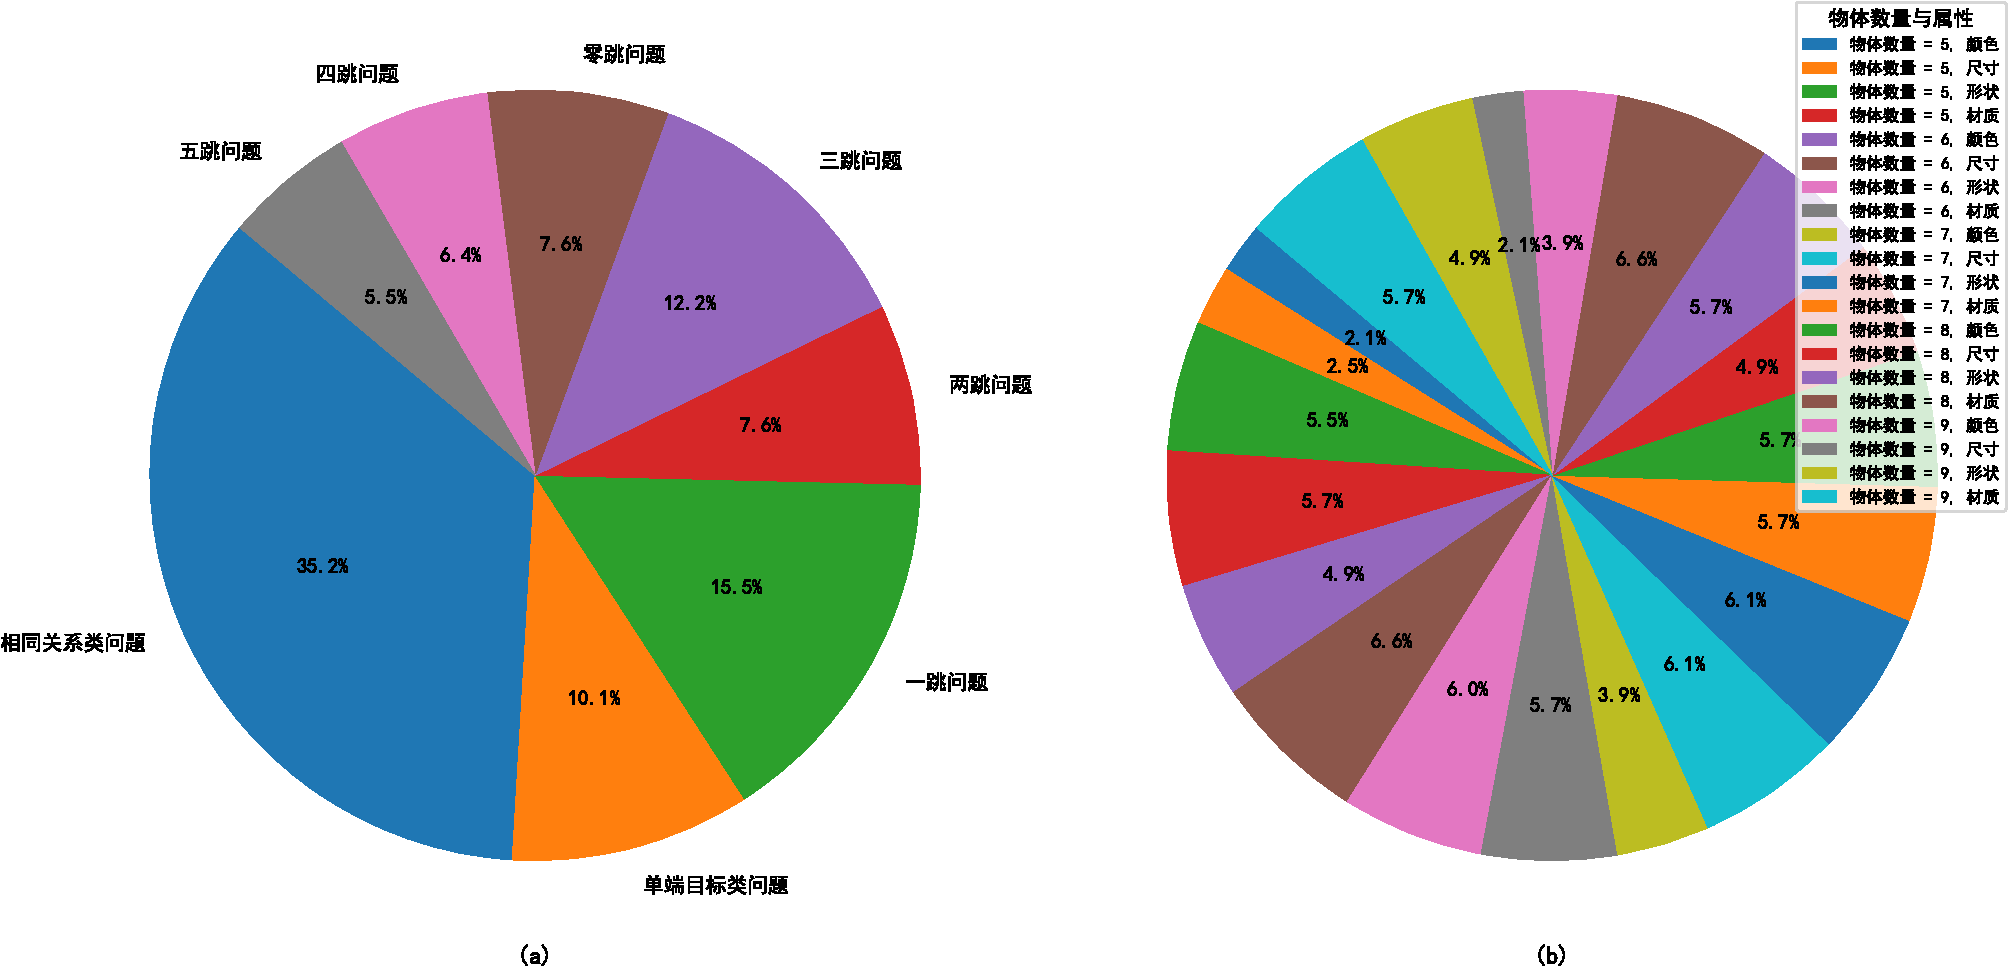
\includegraphics[scale=0.45]{figures/question_template_distribution-crop.pdf}
    \caption{(a)为问题模板分布,(b)查询属性在物体数量为5到9之间的分布}
    \label{fig:template_statistics}
\end{figure}

问题分布的统计图见图\ref{fig:question_statistics}(a)。从统计图中可得知,有关颜色和形状的问题在POVQAD数据集中
占比最高,分别是39\%和37.6\%,关于大小和材质的问题则相对较少,分别只占到了13.6\%和9.8\%。
所提问题的类型取决于被查询的物体的属性,在生成数据集的过程中,允许用户设置问题类型的预期占比。
以上问题类型占比,是基于以下的设置生成的:颜色问题占比40\%,形状问题占比40\%,大小问题占比10\%,材质问题占比10\%。
做出如上设置的原因是,与材质(只有两个值)相比,颜色和形状等属性包含更大的值集合(颜色有 8 个值,形状有 4 个值)。
因此,以颜色为中心的问题的答案集空间比以材质为中心的问题的答案集空间更广,从而为数据集带来了更多样化的答案集空间。

图\ref{fig:question_statistics}(b)、(c)、(d)和(e)分别说明了各种问题类型(尺寸、形状、材质和颜色)的潜在答案的分布。
生成数据集的目标之一是实现均衡的分布,避免大多数问题都导致相同的答案集的情况。
例如,当问题涉及物体的大小时,其可能的解可以是
 {大, 中}、{大, 小}、{小, 中}、{大}、{中} 或 {小} 之一,
 如图\ref{fig:question_statistics}(b)所示。由于查询属性为颜色的问题的可能答案数量很大(因为颜色可以取 8 个值),
 因此图\ref{fig:question_statistics}(e)中并未列出整个空间。根据统计图可以看出,在生成过程中没有偏向任何特定的答案。
\begin{figure}[h]
    \centering
    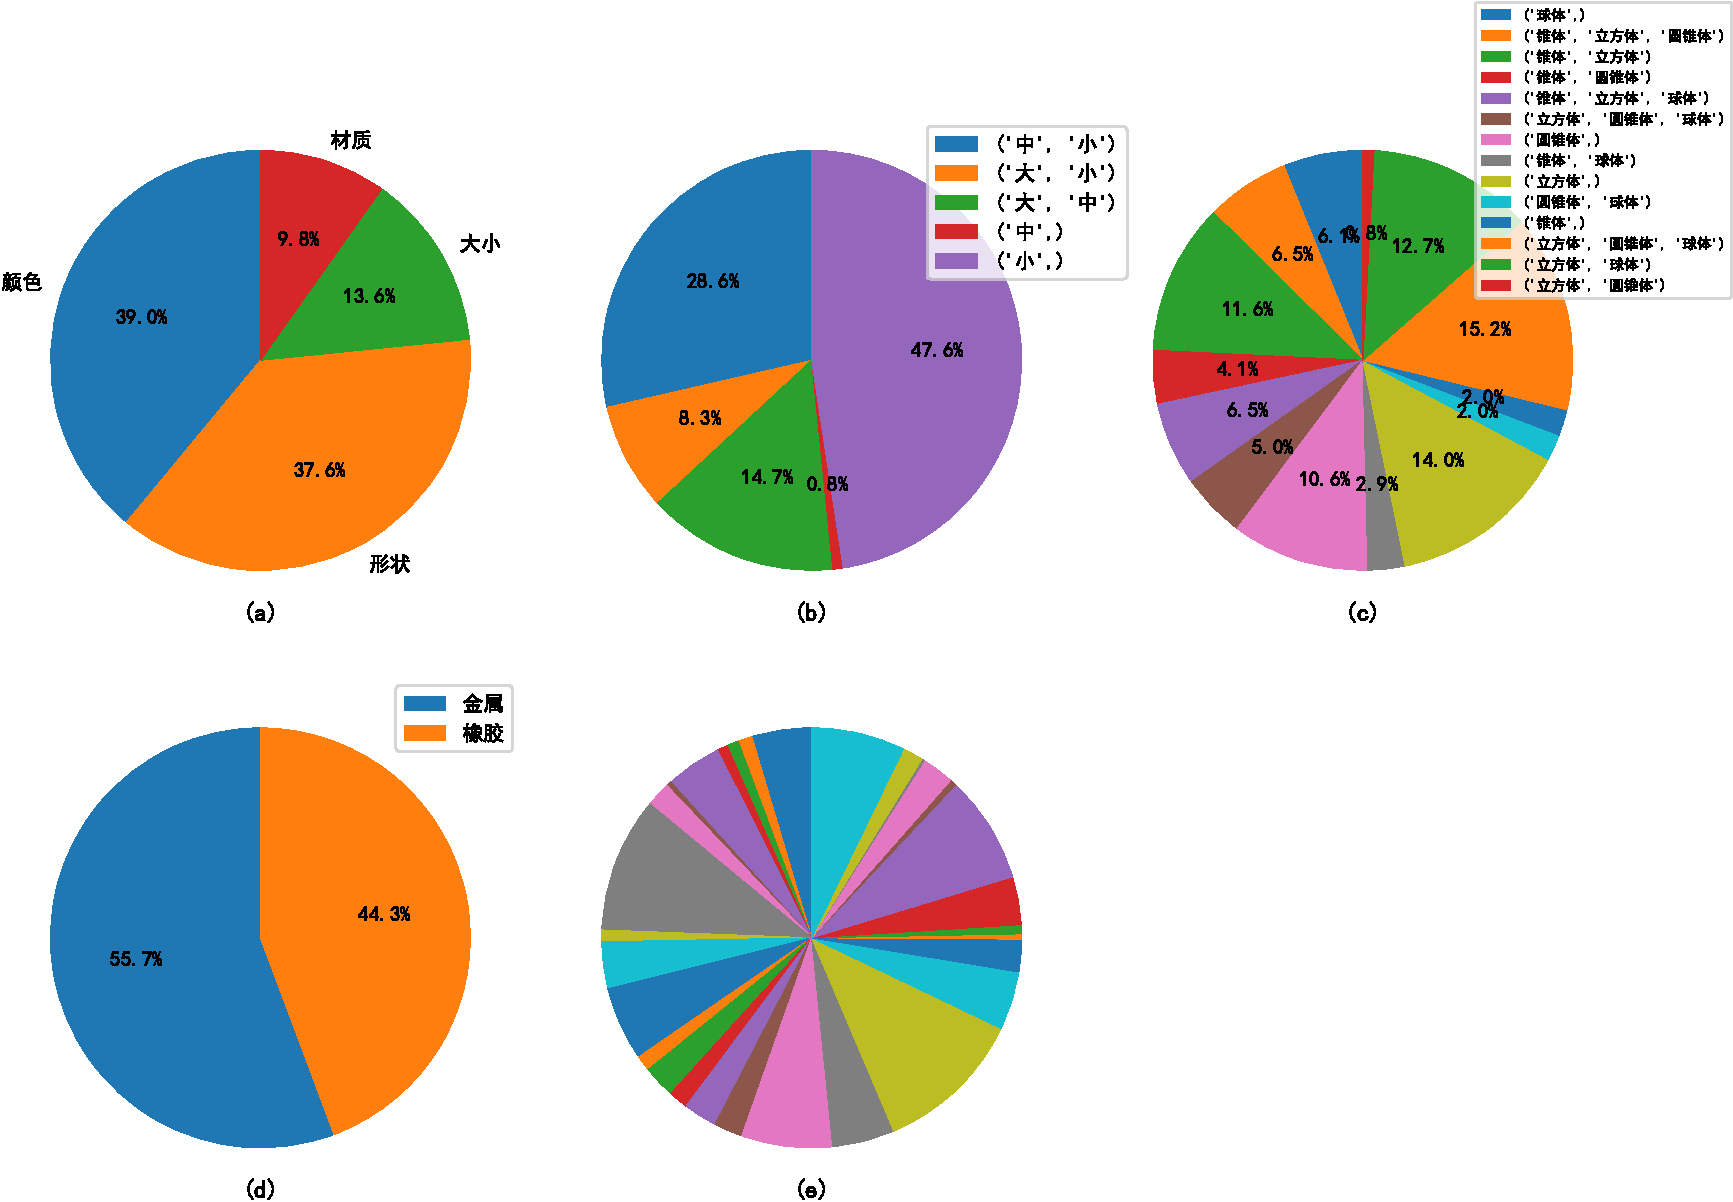
\includegraphics[width=\textwidth]{figures/question_distribution-crop.pdf}
    \caption{(a)问题类型分布;(b) 查询属性为尺寸的问题的答案分布;(c)查询属性为材质的问题的答案的分布;(d)查询属性为形状的问题的答案的分布;(e)查询属性为颜色的问题的答案的分布。由于这些问题的可能的答案数较多(> 100),故此处未列出}
    \label{fig:question_statistics}
\end{figure}
\section{实验与评估}
\subsection{质量分析}
\subsubsection{质量保证}
为了保证数据集的质量,采用双盲审核机制,邀请两名评审员各自独立对数据集进行评审,验证每个问题
的答案、推理解答所需步数及问题是否可观察。在评审过程中,如果两名评审员同时判定该问题出现错误,那么
将该问题剔除。双盲评审的结果见表\ref{tab:kappa},其中展示了评审员1和评审员2分别与初始标注的一致性,以及两名评审员
之间的一致性。通过Fleiss's Kappa衡量的评审员间的一致性超过0.8,证明了数据集的可靠性。
\begin{table}[h]
    \centering
    \renewcommand{\arraystretch}{0.8}
    \begin{tabular}{lccc}
    \toprule
     & \makecell{答案是否正确} & \makecell{推理所需步数} & \makecell{问题是否可观察}\\
    \midrule
    初始标注与评审员1 & 81.2 & 84.4 & 89.6 \\
    初始标注与评审员2 & 84.2 & 85.6 & 85.4 \\
    评审员1与评审员2 & 80.1 & 83.8 & 86.9 \\
    \midrule
    平均值 & 81.8 & 84.6 & 87.3 \\
    \bottomrule
    \end{tabular}
    \caption{评审员1、2和初始标注之间的标注者间一致性}
    \label{tab:kappa}
\end{table}
\subsubsection{难度保证}
本文通过记录2位评审员在POVQAD数据集上回答问题时的正确率、以及所需检索信息的次数、回答问题所需要的跳数,来对
数据集的难度进行判断,并于其它现有的VQA数据集进行比较。实验结果见表\ref{tab:human_performance},其中明显可以看出,POVQAD回答问题所需
的跳数,明显大于现有数据集VQAv2,另外POVQAD所需的检索信息的次数也更多一些,这些都证明了回答POVQAD数据集
所需的外部知识更多,考虑次数更多,数据集难度更大。另外,人类在本文
构造的POVQAD数据集上的准确率最低,进一步侧面印证了本文构造数据集的挑战性。
\begin{table}[h]
    \centering
    \renewcommand{\arraystretch}{0.8}
    \begin{tabular}{lccc}
    \toprule
     & \makecell{回答问题正确率} & \makecell{推理所需跳数} & \makecell{检索信息次数}\\
    \midrule
    POVQAD & 81.2 & 84.4 & 89.6 \\
    CLEVR & 84.2 & 85.6 & 85.4 \\
    GQAv2 & 80.1 & 83.8 & 86.9 \\
    \midrule
    平均值 & 81.8 & 84.6 & 87.3 \\
    \bottomrule
    \end{tabular}
    \caption{人类评审员在不同VQA数据集上回答问题的表现}
    \label{tab:human_performance}
\end{table}

\section{本章小结}
本章围绕POVQAD(Partial Observation VQA Dataset)数据集的设计与构建进行了系统介绍。
该数据集以CLEVR为基础,借鉴现实中信息不可完全观测的特点,引入了部分可见性、遮挡机制和复杂环境约束,
以更真实地模拟智能体在真实物理世界中所面临的推理挑战。

在设计目标方面,POVQAD明确提出要评估和提升模型在部分可见条件下的空间推理能力,
并通过引入区域属性与逻辑约束(使用ASP表示)为推理过程提供先验结构支持。在构建流程上,数据集经历了从环境生成、完整场景图生成、
部分场景图生成、问题与答案生成,再到图像渲染与表示转换的完整技术路径,确保数据在逻辑一致性、多样性与推理复杂性之间实现平衡。

此外,本章通过统计分析展示了问题模板、属性分布与答案空间的覆盖情况,证明了数据集在任务类型和解集结构上的均衡性。
质量评估与难度评估实验进一步佐证了数据集在标注一致性、问题合理性及推理复杂度等维度的高标准,
验证了POVQAD作为研究神经符号推理系统的重要基准集的实用价值和挑战性。

本章为后续神经符号VQA框架在复杂视觉问答任务中的实验与分析奠定了坚实的数据基础。